%%%%%%%%%%%%%%%%%%%%%%%%%%%%%%%%%%%%%%%%%
% University Assignment Title Page 
% LaTeX Template
% Version 1.0 (27/12/12)
%
% This template has been downloaded from:
% http://www.LaTeXTemplates.com
%
% Original author:
% WikiBooks (http://en.wikibooks.org/wiki/LaTeX/Title_Creation)
%
% License:
% CC BY-NC-SA 3.0 (http://creativecommons.org/licenses/by-nc-sa/3.0/)
% 
% Modified for COSC480/490 by:
% Lech Szymanski (8/3/18)

\documentclass[12pt]{article}
\usepackage[draft]{cosc4x0style}

% To compile the final version of the report (which will remove all the todo content)
%\usepackage{cosc4x0style}

% Specify project code 480 or 490
\papercode{385}

% Your project title
\title{Verlan Identification with LLMs}

% Your name
\author{Yitian \textsc{Li}}
\studentid{4556502}

% Names of your supervisors, separated by line break '\\'
\supervisors{
  Dr. Lech \textsc{Szymanski} \\
  Dr. Veronica \textsc{Liesaputra}
}

% Date, change the \today to a set date if you want to be precise
\reportdate{\today}

\begin{document}


\maketitle

\begin{abstract}
An abstract summarises, in one paragraph, the major aspects of the entire work. It usually highlights the overall purpose/aim of the project, the research problem(s) studied, the approach and the results.
\end{abstract}

\section{Introduction}

Introduce the project, its major aims and summary of the findings (try not to just repeat the abstract). For example, the purpose of this document is to provide a template for your report with examples of commonly used \LaTeX{} commands and features. Naturally, your introduction should not be as brief as this.
 
\section{Background}

Typically, introduction will be followed with a section providing the background for the project. This often means a bit of literature review or explanation of the fundamental concepts/terminology. This section has a dual purpose: 
\begin{itemize}
\item to provide enough information for the readers, who might not be experts in your field, so that they can understand everything that follows - methods, results, etc.;
\item to demonstrate that you have gained a sufficient level of competency in the topic.
\end{itemize}

Don't forget to cite the sources of your information. For instance, a reference for \LaTeX{} can be found here \cite{latexcompanion}. If you were, say, interested in Computer Vision you might want to take a look at this article \cite{bettersift}. If you want to cite two related document at once, you can do it like so \cite{bettersift,sift}.

\section{How to compile \LaTeX{}}

The remaining sections should present what you have done in your project including the results and analysis. For this document, this will be a demonstration of how to use \LaTeX{} in order to create your report. 

\LaTeX{} documents are prepared using markup language and need to be compiled to produce pdfs. 

The easiest way is to use the \href{https://www.overleaf.com}{Overleaf service} - it's free for private projects. Create an account and once you login you can create different projects (essentially different documents). If you joined the ``COSC4x0 Report Template project" by following the link from Blackboard, you can \textit{Copy} and rename it to create a new project from your Overleaf \textit{Home} page. Alternately, you can click the ``New Project" button, select the ``Upload project" option and upload the \textit{cosc4x0report.zip} file where this pdf came from. The template will open on the website and you'll be able to edit the report in your browser, compile LaTeX to pdf online and have it saved on a remote server. Later you just download the final pdf and submit as your report.   

Another option is to install a LaTeX compiler on your machine and compile the .tex file yourself. On macOS you need to download and install \href{http://www.tug.org/mactex/downloading.html}{MacTeX}. Then, using programs like \href{http://pages.uoregon.edu/koch/texshop/}{TexShop} (free), or VSCode (with appropriate extensions) (also free), or \href{https://www.texifier.com/}{Texifier} (awesome, but not free) you can edit and compile a .tex file into a .pdf.

\section{\LaTeX{} markup examples}
\label{sec:examples}
 
\subsection{Sections}

Use \verb$\section{}$ and \verb$subsection{}$ commands to organise your document. \LaTeX{} handles all the formatting and numbering automatically. Use \verb$\label{}$ and \verb$\ref{}$ commands for cross-references.

\subsection{Comments}

Comments might be useful during the writing process, as reminders or questions to your supervisor (who should get a chance to comment on your report). Comments can be added to the margins of the document using the \todo{Here's a comment in the margin!} \verb$\todo{}$ command, as shown in the example on the right. You can also add inline comments:

\todo[inline, color=green!40]{This is an inline comment.}

\subsection{Tables and Figures}

Use the \verb$table{}$ and \verb$\tabular{}$ commands for basic tables --- see Table~\ref{tab:widgets}, for example. You can include a figure (JPEG, PNG or PDF) with the \verb$\includegraphics{}$ command as in the code for Figure~\ref{fig:frog} below.

% Commands to include a figure:
\begin{figure}
\centering
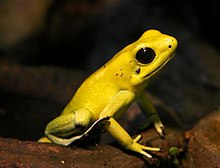
\includegraphics[width=0.5\textwidth]{figures/frog.jpg}
\caption{\label{fig:frog}This is a figure caption.}
\end{figure}

\begin{table}
\centering
\begin{tabular}{l|r}
Item & Quantity \\\hline
Widgets & 42 \\
Gadgets & 13
\end{tabular}
\caption{\label{tab:widgets}An example table.}
\end{table}

\subsection{Mathematics}

\LaTeX{} is great at typesetting mathematics. Let $X_1, X_2, \ldots, X_n$ be a sequence of independent and identically distributed random variables with $\text{E}[X_i] = \mu$ and $\text{Var}[X_i] = \sigma^2 < \infty$, and let
\begin{equation}S_n = \frac{X_1 + X_2 + \cdots + X_n}{n}
      = \frac{1}{n}\sum_{i}^{n} X_i\label{my_eq1}\end{equation}
denote their mean. Then as $n$ approaches infinity, the random variables $\sqrt{n}(S_n - \mu)$ converge in distribution to a normal $\mathcal{N}(0, \sigma^2)$. You can also reference labeled equations, such as Equation~\ref{my_eq1}.

\subsection{Lists}

You can make lists with automatic numbering \dots

\begin{enumerate}
\item Like this,
\item and like this.
\end{enumerate}
\dots or bullet points \dots
\begin{itemize}
\item Like this,
\item and like this.
\end{itemize}

\section{Conclusion}

Concluding remarks. Send the pdf (not the \verb$*.tex$ file) to your supervisor for comments (as early as possible). Don't forget to change the\\ \verb$\usepackage[draft]{cosc4x0style}$ setting to\\ \verb$\usepackage{cosc4x0style}$ to produce the pdf in the format for the final submission.

%The environment \thebibliography produces a list of references; such list will be titled "References". A parameter inside braces, 9 in the example, indicates the number of entries to be added; this parameter can not be greater than 99.

%To create a bibliography entry the command \bibitem is used. A parameter inside braces is set to label this entry and can later be used as identifier for this reference. After the closing brace the text with the name of the author, the book title, publisher and so on is entered. 

%Any choice of citation style is acceptable as long as you are consistent.

\begin{thebibliography}{9}

\bibitem{latexcompanion} 
Michel Goossens, Frank Mittelbach, and Alexander Samarin. \textit{The \LaTeX\ Companion}. Addison-Wesley, Reading, Massachusetts, 1993.

\bibitem{bettersift}
Nabeel Khan, Brendan McCane, and Steven Mills. \textit{Better Than SIFT?}. Machine Vision and Applications, 26(6):819--836, 2015.

\bibitem{sift}
D. G. Lowe. \textit{Distinctive image features from scale invariant key-points}. International Journal of Computer Vision, 60, 91–-110, 2004.

\end{thebibliography}


% Activate the appendix
% from now on sections are numerated with capital letters
\appendix

\renewcommand{\thesection}{Appendix \Alph{section}}

\section{Some extra things}

If you have anything more to add such as:
\begin{itemize}
\item not essential details - things that might be too much for first time reading, or could be distracting from the main points...but are still important for reproducibility or deeper understanding
\item work that was done in the project but doesn't go with the main work, or detracts/is not essential for the main narrative.  
\end{itemize}

\section{Aims and Objectives}

\textbf{Interim report only!} -- you do not need to include this appendix in the final report.  However, in your interim the last appendix should include your original Aims and Objectives, and, if the things have changed, the revised Aims and Objectives. If you used the \LaTeX{} template provided for your Aims and objectives document, just copy the \verb$\paragraph{Aims}$ and \verb$\paragraph{Objectives}$ sections and paste them here.

\subsection*{Original}

\paragraph{Aims}
Here you are describing the term goal of the project. What do you want to achieve by the end?  What is the ultimate goal of this work?  For example, the primary aim of this document is to have students produce suitable aims and objectives for their COSC480/490 project. While the aims and objectives document is not an assessed deliverable, a clear definition of what is to be done, and a bit of planning of how it is to be accomplished is paramount to the project's success. It is important to establish the scope of the project.

\paragraph{Objectives}
Objectives list the milestones that you need to achieve in order to achieve the projects aim(s). It's a rough plan for what needs to happen in what order. It's best to list the objectives in bullet point form. For many projects the structure to these objectives might follow the following pattern (objective names are just examples -- you can have different objective names):    
\begin{itemize}[noitemsep]
\item background reading; going through the literature; learning about the research field;
\item setting up of some kind of system for the project; getting the environment for experiments working;
\item conducting preliminary experiments; implementation of a basic/simple approach; producing base case results;
\item trying method 1; recording the results;
\item trying method 2; recording the results.
\end{itemize}

\subsection*{Revised}

\paragraph{Aims}
Here you are describing the term goal of the project. What do you want to achieve by the end?  What is the ultimate goal of this work?  For example, the primary aim of this document is to have students produce suitable aims and objectives for their COSC480/490 project. While the aims and objectives document is not an assessed deliverable, a clear definition of what is to be done, and a bit of planning of how it is to be accomplished is paramount to the project's success. It is important to establish the scope of the project.

\paragraph{Objectives}
Objectives list the milestones that you need to achieve in order to achieve the projects aim(s). It's a rough plan for what needs to happen in what order. It's best to list the objectives in bullet point form. For many projects the structure to these objectives might follow the following pattern (objective names are just examples -- you can have different objective names):    
\begin{itemize}[noitemsep]
\item background reading; going through the literature; learning about the research field;
\item setting up of some kind of system for the project; getting the environment for experiments working;
\item conducting preliminary experiments; implementation of a basic/simple approach; producing base case results;
\item trying method 1; recording the results;
\item trying method 2; recording the results.
\end{itemize}


\end{document}